\section{Summary}

        Electrohydrodynamic Atomization (EHDA), also known as Electrospray (ES), is a way to disintegrate a liquid into droplets by exposing it to a strong electric field.
EHDA surveys have contributed as an important tool for the development of water technology (thermal desalination and metal recovery), material sciences (nanofibers and nano spheres fabrication, metal recovery, selective membranes, and batteries), and biomedical application (droplet encapsulation).
Besides that, the project is merged with the Energy Transition strategy and Innovation Agenda Agriculture, Water, and Food, Key Enabling Technologies (KETs). 
Although, there are EHDA applications in industry, stabilizing the cone-jet spray mode is done empirically and based on mean current measurements. 

The electric current flowing transported by the spray reveals characteristic shapes for different spray modes.
Those shapes cannot simply be summarized by its mean value. In figure one we can see an example of cone-jet mode electrospray.

\begin{figure}[H]
    \center
    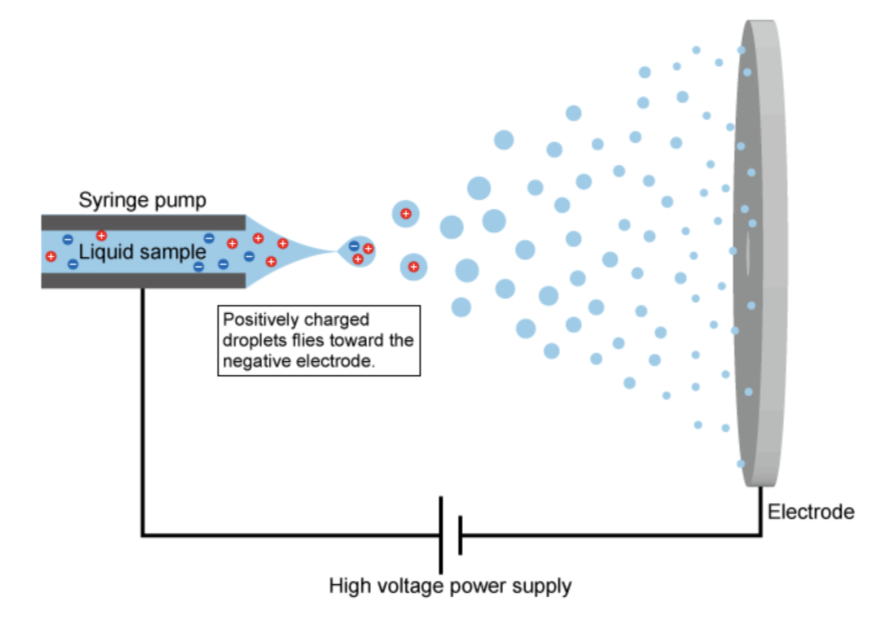
\includegraphics[width=8cm]{images/electrospray.png}
    \label{img1}
    \caption{EHDA}
\end{figure}

Signal processing techniques can allow a non-visual classification of the spray mode based on the electric current shape.
The spray process imposes noise and random sequences on the measured signal making its classification not a trivial task. 

Industrial applications demand automated stabilization of a spray mode.
This can be achieved by a closed-loop control system.
Automated classification of the spray mode is a crucial part of a control system same as the development of an appropriate control algorithm. 
Signal processing implementations of previous projects of the NHL Stenden Water Technology group are showing good classification results.
Further research is necessary to improve the classification accuracy and research and implementation of a suitable classification algorithm. 
Because of that, the work will be done by the Water Technology Group at NHL Stenden University of Applied Sciences and in combination with Dutch companies to match analysis possibilities with knowledge and infrastructure availability.

The setup used for this project can be seen in the Figure 2. To run the experiment automatically it is used a computational processing machine to integrate the peripherals and run their routines, system sensors such as the oscilloscope and the high speed camera 
and also the system actuators which is represented by the high voltage power supply and the syringe pump. 

\begin{figure}[H]
    \center
    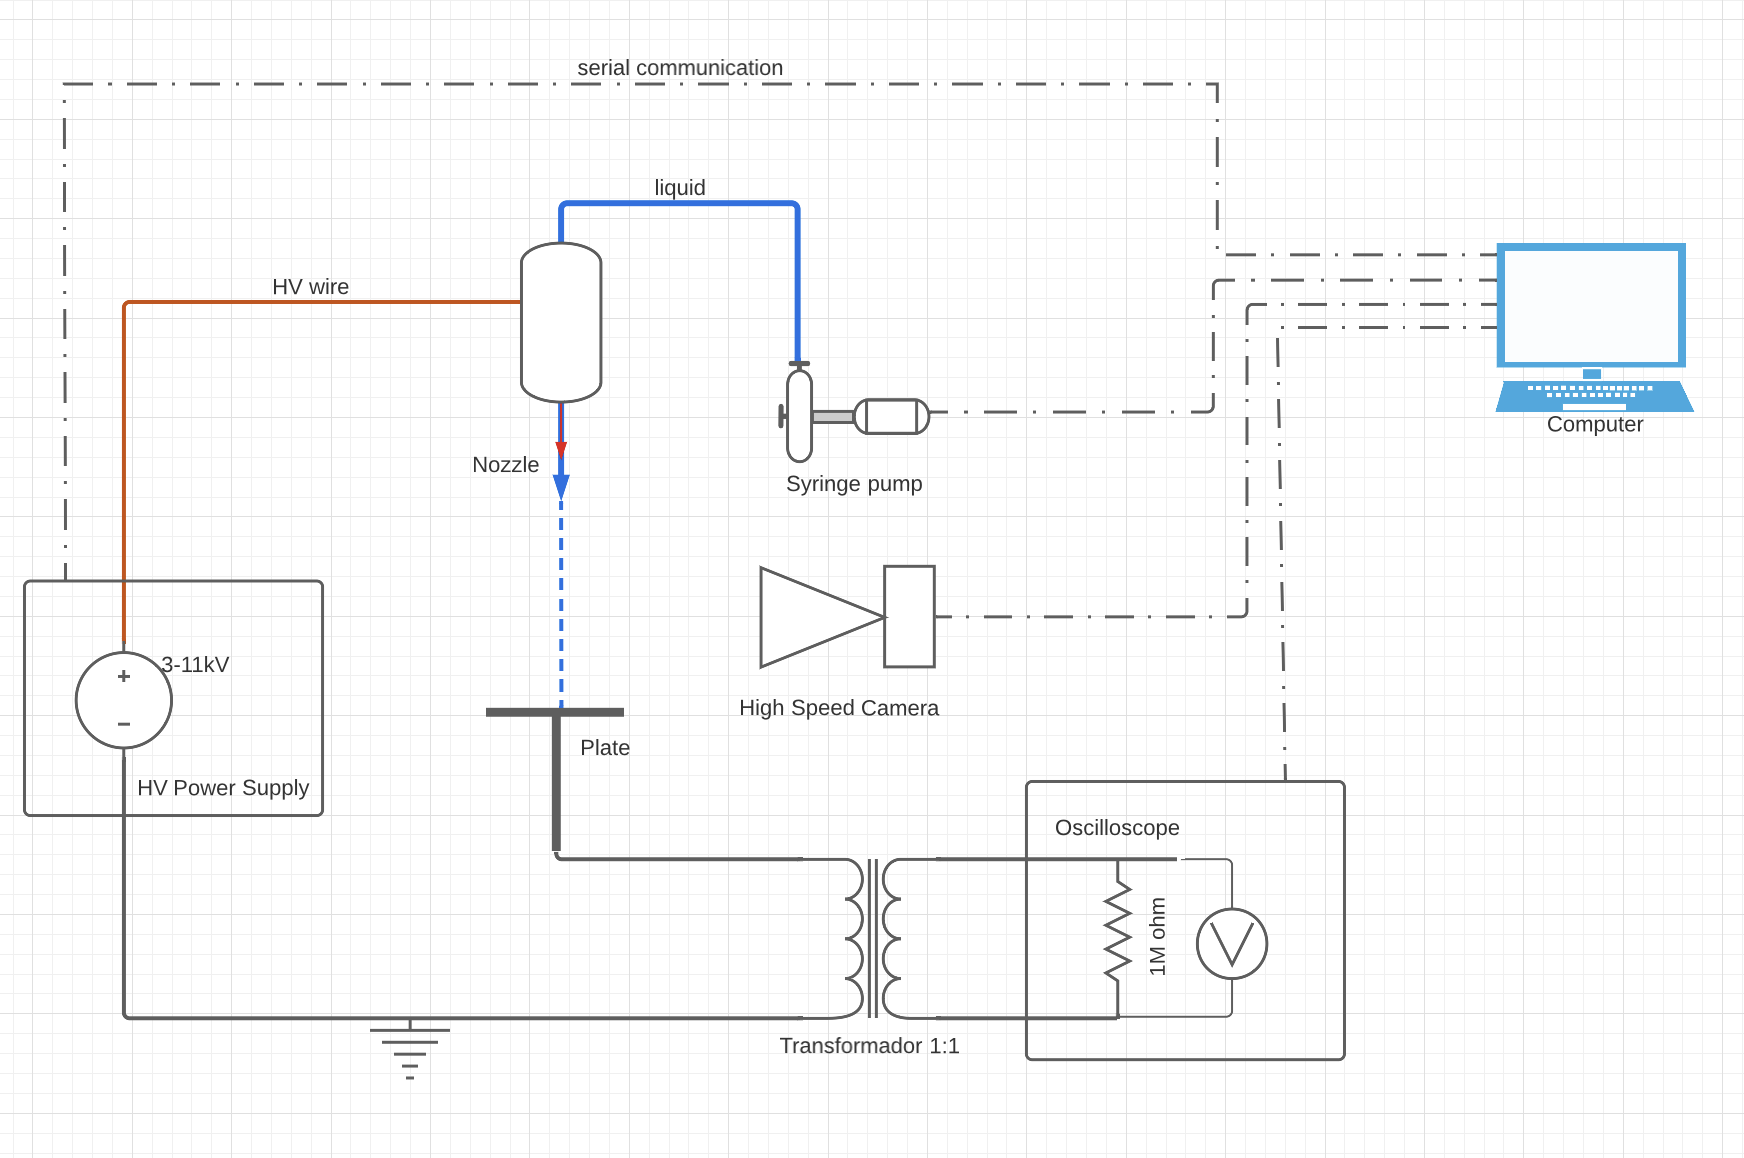
\includegraphics[width=12cm]{images/images_folder_1/system_design.png}
    \caption{System Architecture}
\end{figure}

The algorithms implemented in the computer machine was developed in python by another student and it is already collecting data and classifying the spraying dynamics.
In Figure 3 and Figure 4 shows pictures took by the high speed camera of some of the possible spraying dynamics we can reach. The videos took by the camera is not being used in the classification
algorithm. It is used for manual validation of it.

\begin{multicols}{2}

    \begin{figure}[H]
        \center
        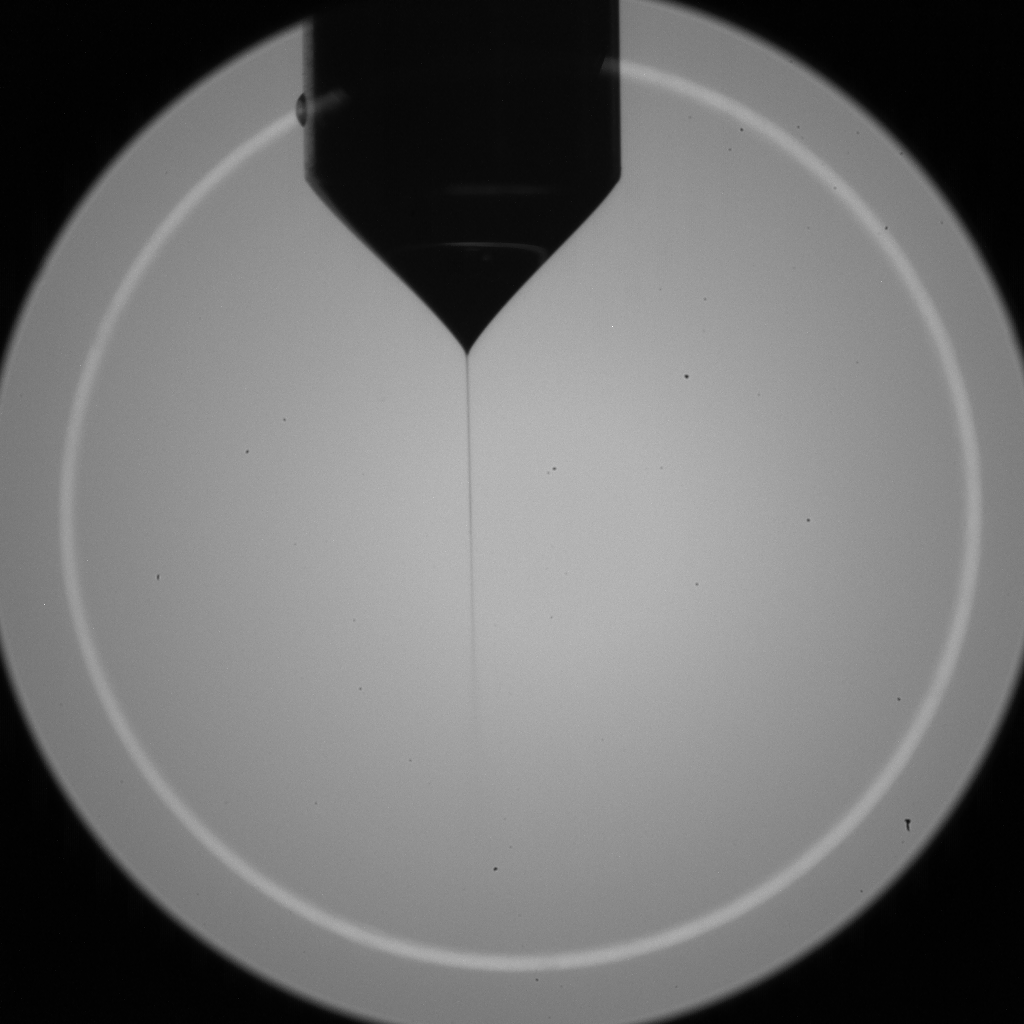
\includegraphics[width=5cm]{images/images_folder_3/conejetexample.png}
        \caption{cone jet mode}
    \end{figure}
    
    \begin{figure}[H]
        \center
        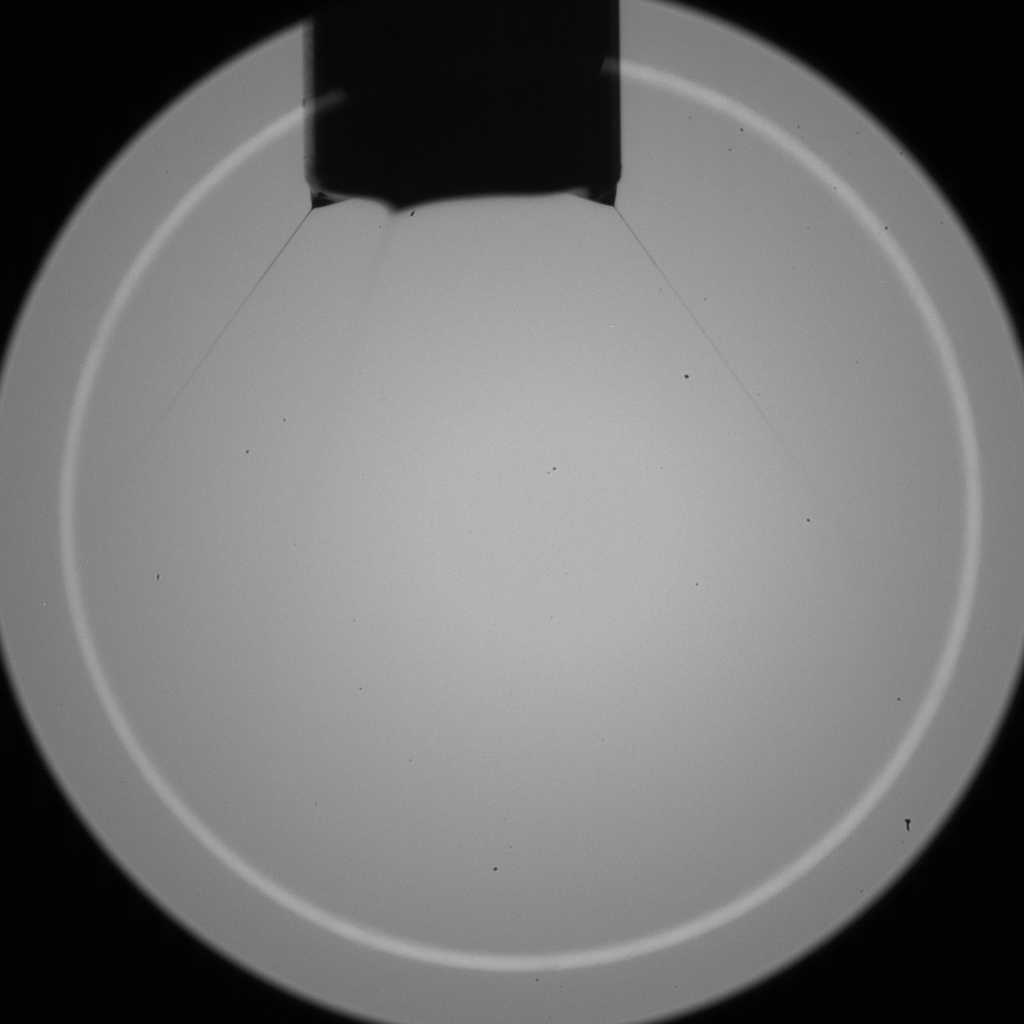
\includegraphics[width=5cm]{images/images_folder_3/multijetexample.png}
        \caption{multi jet mode}
    \end{figure}

    
\end{multicols}
